

%% AAPT Physics Bowl Exams Questions
%%----------------------------------------

%% This section has 14 problems


%% PhysicsBowl 2015
%%----------------------------------------
\element{aapt}{ %% bowl-M1
\begin{question}{bowl-2015-q01}
    Which one of the following choices correctly represents a length of \SI{3.00}{\milli\meter}?
    \begin{multicols}{2}
    \begin{choices}
        \wrongchoice{\SI{3.00e-6}{\meter}}
      \correctchoice{\SI{3.00e-3}{\meter}}
        \wrongchoice{\SI{3.00e-2}{\meter}}
        \wrongchoice{\SI{3.00e3}{\meter}}
        \wrongchoice{\SI{3.00e6}{\meter}}
    \end{choices}
    \end{multicols}
\end{question}
}

\element{aapt}{ %% Bowl-M1
\begin{question}{bowl-2015-q11}
    Two length measurements are made and recorded as
        $L_1=\SI{84.55}{\centi\meter}$ and $L_2=\SI{33.55}{\centi\meter}$.
    Two other length measurements are made and recorded as
        $L_3=\SI{1.750}{\centi\meter}$ and $L_4=\SI{1.250}{\centi\meter}$.
    These measurements are used to compute the quantity
        $\left( L_1 + L_2\right)-\left(L_3 + L_4\right)$ using the rules of significant figures.
    Which one of the following choices best represents the correct result to this calculation?
    \begin{multicols}{2}
    \begin{choices}
        \wrongchoice{\SI{115.100}{\centi\meter}}
      \correctchoice{\SI{115.10}{\centi\meter}}
        \wrongchoice{\SI{115.1}{\centi\meter}}
        \wrongchoice{\SI{115}{\centi\meter}}
        \wrongchoice{\SI{120}{\centi\meter}}
    \end{choices}
    \end{multicols}
\end{question}
}


%% PhysicsBowl 2014
%%----------------------------------------
\element{aapt}{ %% Bowl-M1
\begin{question}{bowl-2014-q02}
    In the laboratory, a student makes the following six measurements for the length of an object: \SI{5.05}{\centi\meter},
        \SI{5.06}{\centi\meter}, \SI{5.07}{\centi\meter}, \SI{5.07}{\centi\meter}, and \SI{5.09}{\centi\meter}.
    Using the rules of significant digits, which one of the following choices correctly represents how she should express the average length of the object?
    \begin{multicols}{3}
    \begin{choices}
        \wrongchoice{\SI{5}{\centi\meter}.}
        \wrongchoice{\SI{5.06}{\centi\meter}.}
        %\wrongchoice{\SI[parse-numbers=false]{5.0\bar{66}}{\centi\meter}.}
        \wrongchoice{\SI{5.066}{\centi\meter}.}
      \correctchoice{\SI{5.07}{\centi\meter}.}
        \wrongchoice{\SI{5.1}{\centi\meter}.}
    \end{choices}
    \end{multicols}
\end{question}
}

\element{aapt}{ %% Bowl-M1
\begin{question}{bowl-2014-q18}
    A rectangular block of wood has a mass of \SI{17.8}{\gram} and dimensions of length: \SI{3.00}{\centi\meter},
        width: \SI{4.00}{\centi\meter}, and height: \SI{2.00}{\centi\meter}.
    Which one of the following choices correctly gives the average density of the block?
    \begin{multicols}{2}
    \begin{choices}
        \wrongchoice{\SI{7.42e5}{\kilo\gram\per\meter\cubed}}
      \correctchoice{\SI{7.42e2}{\kilo\gram\per\meter\cubed}}
        \wrongchoice{\SI{7.42}{\kilo\gram\per\meter\cubed}}
        \wrongchoice{\SI{7.42e-1}{\kilo\gram\per\meter\cubed}}
        \wrongchoice{\SI{7.42e-4}{\kilo\gram\per\meter\cubed}}
    \end{choices}
    \end{multicols}
\end{question}
}


%% PhysicsBowl 2013
%%----------------------------------------
\element{aapt}{ %% Bowl-M1
\begin{question}{bowl-2013-q01}
    Red light from a laser is noted to have a wavelength of
        \SI{632.8}{\nano\meter}.
    Which one of the following choices best represents the
        meaning of the prefix \emph{nano}?
    \begin{multicols}{3}
    \begin{choices}
        \wrongchoice{\num{e-3}}
        \wrongchoice{\num{e-6}}
      \correctchoice{\num{e-9}}
        \wrongchoice{\num{e-12}}
        \wrongchoice{\num{e-15}}
    \end{choices}
    \end{multicols}
\end{question}
}

\element{aapt}{ %% Bowl-M1
\begin{question}{bowl-2013-q13}
    Which one of the following choices represents the measurement with the most number of significant digits?
    \begin{multicols}{2}
    \begin{choices}
        \wrongchoice{\SI{6.75}{\meter}}
        \wrongchoice{\SI{4.67e9}{\meter}}
        \wrongchoice{\SI{0.000 000 012}{\meter}}
        \wrongchoice{\SI{8100}{\meter}}
      \correctchoice{\SI{2.000 05}{\meter}}
    \end{choices}
    \end{multicols}
\end{question}
}


%% PhysicsBowl 2012
%%----------------------------------------
\element{aapt}{ %% Bowl-M1
\begin{question}{bowl-2012-q01}
    Which one of the following lengths is the largest?
    \begin{multicols}{2}
    \begin{choices}
        \wrongchoice{one centimeter}
      \correctchoice{one kilometer}
        \wrongchoice{one millimeter}
        \wrongchoice{one meter}
        \wrongchoice{one nanometer}
    \end{choices}
    \end{multicols}
\end{question}
}

\element{aapt}{ %% Bowl-M1
\begin{question}{bowl-2012-q03}
    Which one of the following choices best represents the value of the speed of light?
    \begin{choices}
        \wrongchoice{\SI{5.90e12}{\mile\per\week}}
      \correctchoice{\SI{1.13e11}{\mile\per\week}}
        \wrongchoice{\SI{1.61e10}{\mile\per\week}}
        \wrongchoice{\SI{6.75e8}{\mile\per\week}}
        \wrongchoice{\SI{1.13e8}{\mile\per\week}}
    \end{choices}
\end{question}
}

\element{aapt}{ %% Bowl-M1
\begin{question}{bowl-2012-q05}
    A solid rectangular box is measured to have length $L=\SI{13.34}{\centi\meter}$,
        width $W=\SI{8.45}{\centi\meter}$, and height $H=\SI{3.36}{\centi\meter}$.
    Which one of the following choices best represents the volume of the box using proper significant digits?
    \begin{multicols}{2}
    \begin{choices}
        \wrongchoice{\SI{4e2}{\centi\meter\cubed}}
        \wrongchoice{\SI{3.8e2}{\centi\meter\cubed}}
      \correctchoice{\SI{3.79e2}{\centi\meter\cubed}}
        \wrongchoice{\SI{3.787e2}{\centi\meter\cubed}}
        \wrongchoice{\SI{3.7875e2}{\centi\meter\cubed}}
    \end{choices}
    \end{multicols}
\end{question}
}

\element{aapt}{ %% Bowl-M1
\begin{question}{bowl-2012-q37}
    The cylindrical head of an aluminum nail has a diameter of \SI{1.00}{\centi\meter}.
    For the top layer of atoms in the nail's head,
        which one of the following choices best represents the number of aluminum atoms in that layer?
    \begin{multicols}{3}
    \begin{choices}
        \wrongchoice{\num{e10}}
      \correctchoice{\num{e15}}
        \wrongchoice{\num{e20}}
        \wrongchoice{\num{e25}}
        \wrongchoice{\num{e30}}
    \end{choices}
    \end{multicols}
\end{question}
}

\element{aapt}{ %% Bowl-M1
\begin{question}{bowl-2012-q46}
    There is a quantity called the Planck time, $t_{planck}$,
        which is computed in terms of constants as $t^2_{planck} = \frac{\hbar G}{c^n}$ where $\hbar$ is Planck's constant divided by $2\pi$,
        $G$ is the Universal Gravitational Constant,
        and $c$ is the speed of light.
    In order for this expression for time to be consistent,
        what is the numerical value of $n$,
        the power to which the speed of light is raised?
    \begin{multicols}{3}
    \begin{choices}
        \wrongchoice{\num{2}}
        \wrongchoice{\num{3}}
        \wrongchoice{\num{4}}
      \correctchoice{\num{5}}
        \wrongchoice{\num{6}}
    \end{choices}
    \end{multicols}
\end{question}
}


%% PhysicsBowl 2011
%%----------------------------------------
\element{aapt}{ %% Bowl-M1
\begin{question}{bowl-2011-q01}
    Which one of the following choices best represents the average mass of an adult human male?
    \begin{multicols}{2}
    \begin{choices}
        \wrongchoice{\SI{1.0e-2}{\kilo\gram}}
        \wrongchoice{\SI{1.0e-1}{\kilo\gram}}
        \wrongchoice{\SI{1.0e1}{\kilo\gram}}
      \correctchoice{\SI{1.0e2}{\kilo\gram}}
        \wrongchoice{\SI{1.0e3}{\kilo\gram}}
    \end{choices}
    \end{multicols}
\end{question}
}

\element{aapt}{ %% Bowl-M1
\begin{question}{bowl-2011-q03}
    The distance of one thousand meters can be written as one kilometer.
    Which one of the following choices best represents a distance of one million meters?
    \begin{choices}
        \wrongchoice{one gigameter (\SI{1}{\giga\meter})}
      \correctchoice{one megameter (\SI{1}{\mega\meter})}
        \wrongchoice{one micrometer (\SI{1}{\micro\meter})}
        \wrongchoice{one nanometer (\SI{1}{\nano\meter})}
        \wrongchoice{one terameter (\SI{1}{\tera\meter})}
    \end{choices}
\end{question}
}

\element{aapt}{ %% Bowl-M1
\begin{question}{bowl-2011-q04}
    The following two measurements of length are recorded from an experiment:
        $L_1=\SI{4.57e3}{\meter}$ and $L_2=\SI{2.130e2}{\meter}$.
    Using the rules of the significant digits,
        what is the sum $\left(L_1+L_2\right)$ of these measurements?
    \begin{multicols}{2}
    \begin{choices}
        \wrongchoice{\SI{5e3}{\meter}}
        \wrongchoice{\SI{4.8e3}{\meter}}
      \correctchoice{\SI{4.78e3}{\meter}}
        \wrongchoice{\SI{4.783e3}{\meter}}
        \wrongchoice{\SI{6.70e3}{\meter}}
    \end{choices}
    \end{multicols}
\end{question}
}


%% PhysicsBowl 2010
%%----------------------------------------
\element{aapt}{ %% Bowl-M1
\begin{question}{bowl-2010-q01}
    The very first PhysicsBowl took place in 1985.
    Approximately how many seconds ago did students compete in this first contest?
    \begin{multicols}{3}
    \begin{choices}
        \wrongchoice{\SI{e2}{\second}}
        \wrongchoice{\SI{e5}{\second}}
        \wrongchoice{\SI{e7}{\second}}
      \correctchoice{\SI{e9}{\second}}
        \wrongchoice{\SI{e12}{\second}}
    \end{choices}
    \end{multicols}
\end{question}
}

\element{aapt}{ %% Bowl-M1
\begin{question}{bowl-2010-q03}
    The following three measurements of length are given:
        $L_1=\SI{22.05}{\meter}$, $L_2=\SI{6.1123}{\meter}$, and $L_3=\SI{89.6}{\meter}$.
    What is the sum of these three measurements using rules of proper significant digits?
    \begin{multicols}{2}
    \begin{choices}
        \wrongchoice{\SI{120}{\meter}}
        \wrongchoice{\SI{118}{\meter}}
      \correctchoice{\SI{117.8}{\meter}}
        \wrongchoice{\SI{117.76}{\meter}}
        \wrongchoice{\SI{117.7623}{\meter}}
    \end{choices}
    \end{multicols}
\end{question}
}


%% PhysicsBowl 2009
%%----------------------------------------
\element{aapt}{ %% Bowl-M1
\begin{question}{bowl-2009-q02}
    A room has a floor area of \SI{25}{\meter\squared}.
    What is this area in \si{\centi\meter\squared}?
    \begin{multicols}{2}
    \begin{choices}
        \wrongchoice{\num{25 000 000}}
      \correctchoice{\num{250 000}}
        \wrongchoice{\num{2 500}}
        \wrongchoice{\num{0.25}}
        \wrongchoice{\num{0.00 25}}
    \end{choices}
    \end{multicols}
\end{question}
}

\element{aapt}{ %% Bowl-M1
\begin{question}{bowl-2009-q04}
    The length measurement $L=\SI{0.01230}{\centi\meter}$ has how many significant digits?
    \begin{multicols}{3}
    \begin{choices}
        \wrongchoice{\num{6}}
        \wrongchoice{\num{5}}
      \correctchoice{\num{4}}
        \wrongchoice{\num{3}}
        \wrongchoice{\num{2}}
    \end{choices}
    \end{multicols}
\end{question}
}


%% PhysicsBowl 2008
%%----------------------------------------
\element{aapt}{ %% Bowl-M1
\begin{question}{bowl-2008-q02}
    In one year, there are approximately \SI{3.15e7}{\second}.
    Which of the following representations using metric prefixes is equivalent to this value?
    \begin{multicols}{3}
    \begin{choices}
        \wrongchoice{\SI{31.5}{\kilo\second}}
      \correctchoice{\SI{31.5}{\mega\second}}
        \wrongchoice{\SI{31.5}{\giga\second}}
        \wrongchoice{\SI{31.5}{\milli\second}}
        \wrongchoice{\SI{31.5}{\pico\second}}
    \end{choices}
    \end{multicols}
\end{question}
}


%% PhysicsBowl 2007
%%----------------------------------------
\element{aapt}{ %% Bowl-M1
\begin{question}{bowl-2007-q01}
    A standard centimeter ruler is shown.
    \begin{center}
    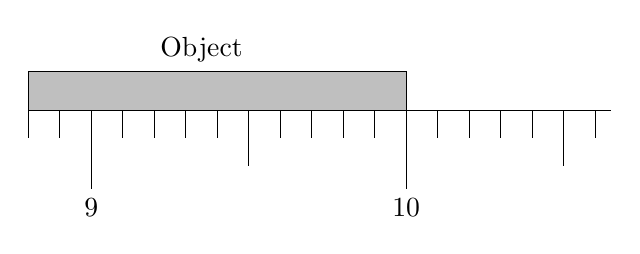
\begin{tikzpicture}
        %% Object
        \draw[fill=white!75!black] (-0.8,0) rectangle (4,0.5);
        \node[anchor=south] at (1.4,0.5) {Object};
        \draw (-0.8,0) -- (6.6,0);
        %% Small Hashes
        \foreach \x in {-8,-4,0,4,8,...,64}{
            \draw (\x mm,0) -- (\x mm,-1em);
        }
        %% Big Hashes
        \foreach \x in {20,40,60}{
            \draw (\x mm,0) -- (\x mm,-2em);
        }
        \draw (0,0) -- (0,-1) node[anchor=north] {$9$};
        \draw (4,0) -- (4,-1) node[anchor=north] {$10$};
    \end{tikzpicture}
    \end{center}
    Which recorded value is the most correct for the location of the shaded object's right end?
    \begin{multicols}{3}
    \begin{choices}
        \wrongchoice{\SI{10}{\centi\meter}}
        \wrongchoice{\SI{10.}{\centi\meter}}
        \wrongchoice{\SI{10.0}{\centi\meter}}
      \correctchoice{\SI{10.00}{\centi\meter}}
        \wrongchoice{$10.\bar{0}$\si{\centi\meter}}
    \end{choices}
    \end{multicols}
\end{question}
}

\element{aapt}{ %% Bowl-M1
\begin{question}{bowl-2007-q02}
    How thick is the average page of a physics textbook?
    \begin{multicols}{3}
    \begin{choices}
        \wrongchoice{\SI{0.1}{\micro\meter}}
        \wrongchoice{\SI{1}{\micro\meter}}
        \wrongchoice{\SI{10}{\micro\meter}}
      \correctchoice{\SI{100}{\micro\meter}}
        \wrongchoice{\SI{1000}{\micro\meter}}
    \end{choices}
    \end{multicols}
\end{question}
}


%% PhysicsBowl 2006
%%----------------------------------------
\element{aapt}{ %% Bowl-M1
\begin{question}{bowl-2006-q01}
    The mass of an object is recorded as $m=\SI{2.10e4}{\kilo\gram}$.
    This mass has been recorded with how many significant digits?
    \begin{multicols}{3}
    \begin{choices}
        \wrongchoice{2}
      \correctchoice{3}
        \wrongchoice{4}
        \wrongchoice{5}
        \wrongchoice{6}
    \end{choices}
    \end{multicols}
\end{question}
}

\element{aapt}{ %% Bowl-M1
\begin{question}{bowl-2006-q02}
    How tall is a flagpole if the sun is at a \ang{53} angle above the horizon and the shadow is \SI{8.0}{\meter} long?
    \begin{multicols}{3}
    \begin{choices}
        \wrongchoice{\SI{4.8}{\meter}}
        \wrongchoice{\SI{6.0}{\meter}}
        \wrongchoice{\SI{8.0}{\meter}}
      \correctchoice{\SI{10.6}{\meter}}
        \wrongchoice{\SI{13.3}{\meter}}
    \end{choices}
    \end{multicols}
\end{question}
}

\element{aapt}{ %% Bowl-M1
\begin{question}{bowl-2006-q11}
    The number of seconds from now until the beginning of the next millennium (year 3000) can be approximate as $10^x$.
    What is $x$?
    \begin{multicols}{3}
    \begin{choices}
        \wrongchoice{$3$}
        \wrongchoice{$4$}
      \correctchoice{$10$}
        \wrongchoice{$30$}
        \wrongchoice{$1000$}
    \end{choices}
    \end{multicols}
\end{question}
}

\element{aapt}{ %% Bowl-M1
\begin{question}{bowl-2006-q12}
    Experimental data are taken.
    Which of the following statements is correct about the precision and accuracy of the data?
    \begin{choices}
        \wrongchoice{If the data are precise, then the data must also be accurate.}
        \wrongchoice{If the data are precise, then the data cannot be accurate.}
        \wrongchoice{If the data are accurate, then the data must also be precise.}
        \wrongchoice{If the data are accurate, then it is not possible for the data to be precise.}
      \correctchoice{The data does not need be either accurate or precise.}
    \end{choices}
\end{question}
}

\element{aapt}{ %% Bowl-M1
\begin{question}{bowl-2006-q21}
    Which of the following is not one of the seven fundamental SI units using the MKS system?
    \begin{multicols}{2}
    \begin{choices}
      \correctchoice{Henry}
        \wrongchoice{Kelvin}
        \wrongchoice{Ampere}
        \wrongchoice{Candela}
        \wrongchoice{Mole}
    \end{choices}
    \end{multicols}
\end{question}
}


%% PhysicsBowl 2005
%%----------------------------------------
\element{aapt}{ %% Bowl-M1
\begin{question}{bowl-2005-q30}
    A scientist measures the dimensions of a rectangular solid to be
        $\SI{1.000}{\milli\meter}\times\SI{20.00}{\centi\meter}\times\SI{5.00}{\centi\meter}$.
    Using proper scientific notation and significant digits,
        what is the volume of the box in units of \si{\meter\cubed}?
    \begin{choices}
        \wrongchoice{\SI{1.000e-5}{\meter\cubed}}
        \wrongchoice{\SI{1.000e-4}{\meter\cubed}}
      \correctchoice{\SI{1.00e-5}{\meter\cubed}}
        \wrongchoice{\SI{1.00e-4}{\meter\cubed}}
        \wrongchoice{\SI{1e-5}{\meter\cubed}}
    \end{choices}
\end{question}
}


\endinput


